\begin{figure}[htb]
  \begin{center}
    \resizebox{\textwidth}{!}{
      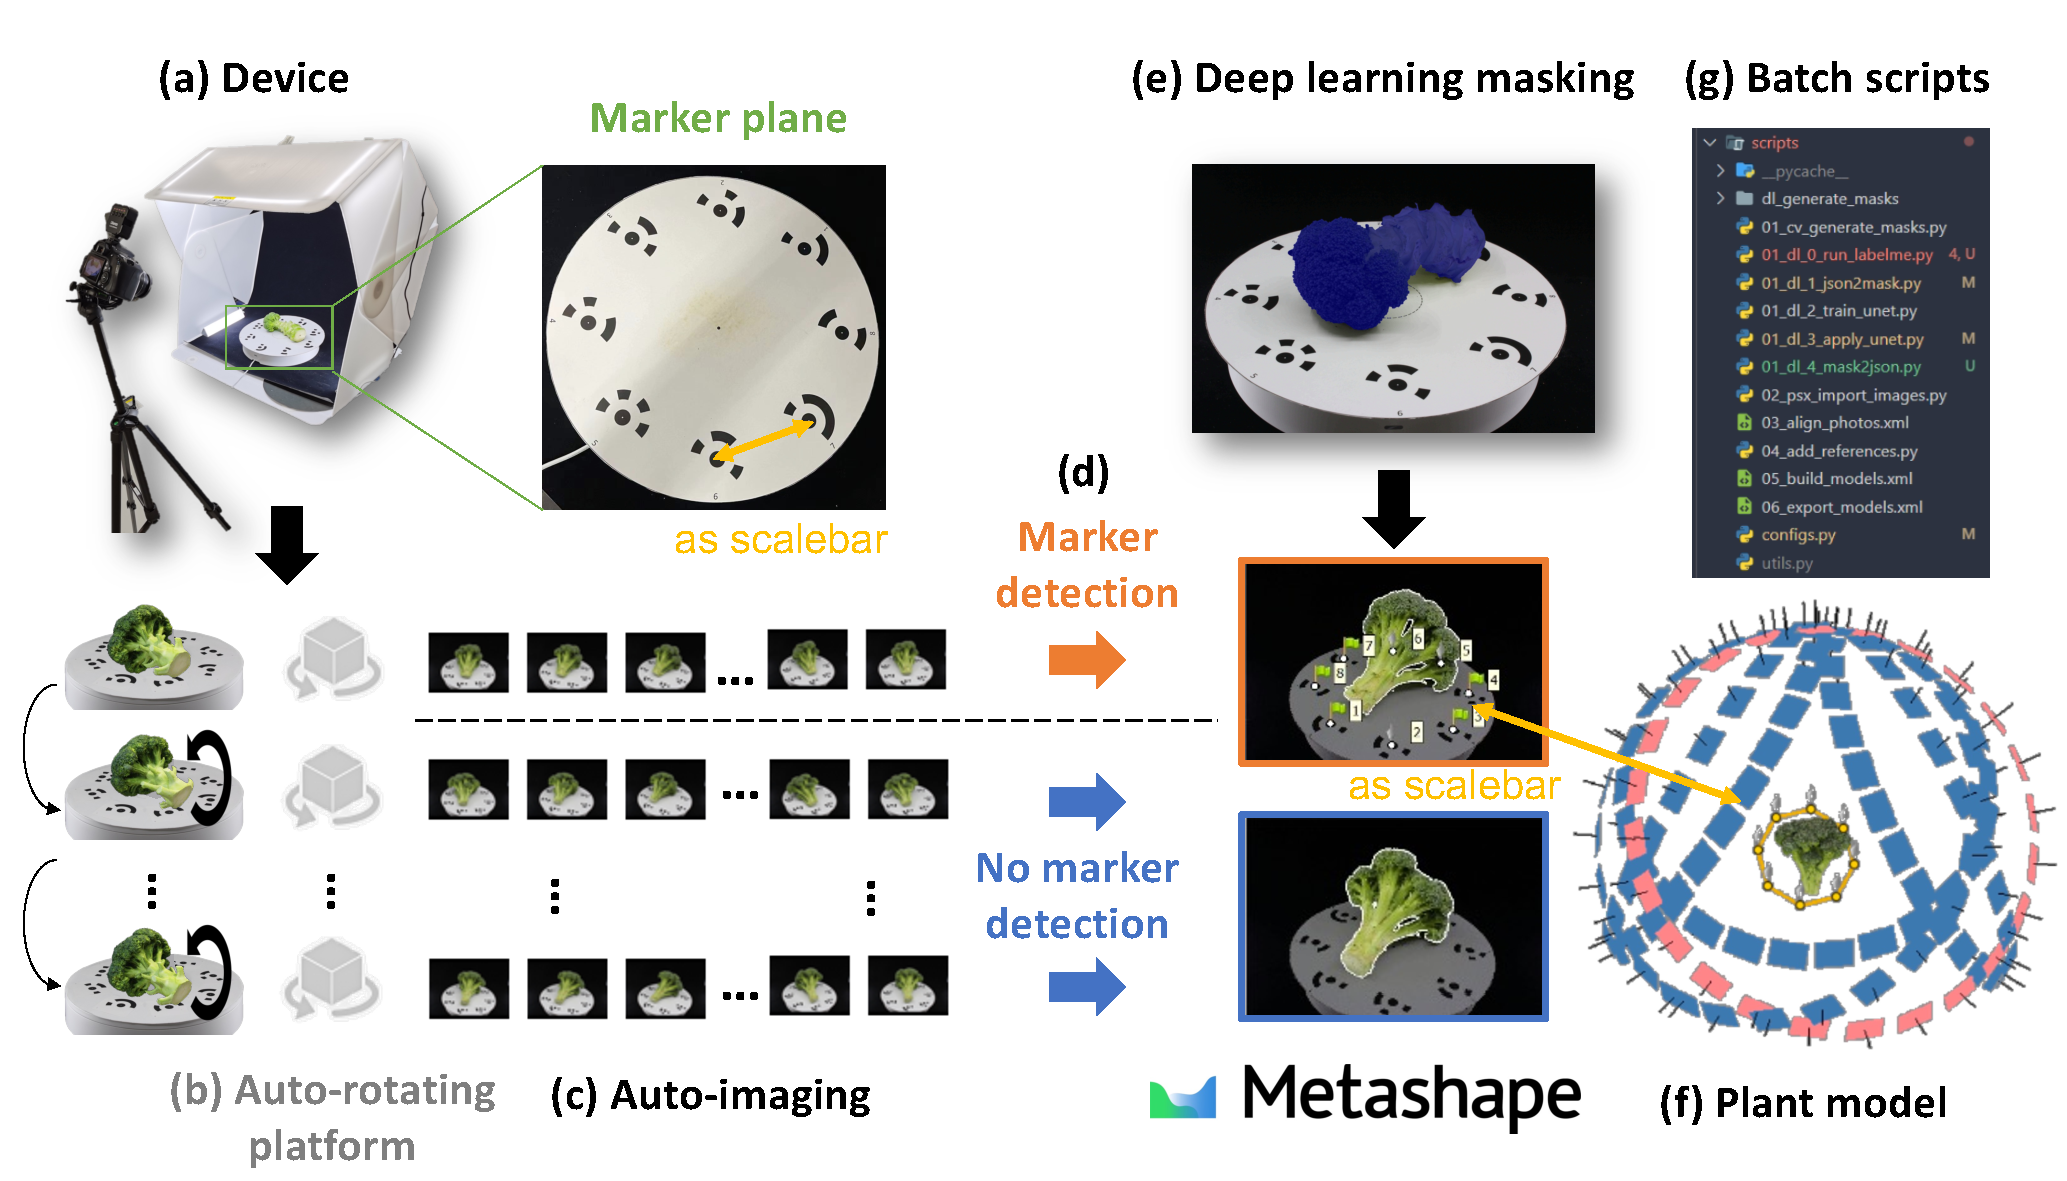
\includegraphics{figures/des/img_recons.pdf}
    }
  \end{center}
  \caption[The plant 3D model reconstruction workflow]{
    The Plant 3D model reconstruction workflow. (a) devices for taking plant images, with a marker plane used as scalebar references; (b) an automatic horizontal rotating platform, which can rotate at a given angle and then stop for a short interval for image taking. The vertical rotation of plants (flip) requires manual operation; (c) different photographic perspectives images taken by the infrared signal auto-imaging system; (d) partial marker detection to avoid misleading image alignment, where only markers on one rotating image group (orange) are detected and not on the others (blue); (e) plant part segmentation using deep learning; (f) the final 3D plant model produced by Metashape; and (g) the scripts for batch processing a large number of plants.
  }
  \label{fig:des_img_recons}
\end{figure}